\documentclass[8pt, a4paper, twoside, twoclumn, english]{extreport}
\usepackage{lipsum, babel}
\usepackage{listings}
\usepackage{graphicx}
\graphicspath{ {./images/} }

\begin{document}

\title{CSCI 415 Assignment 1}
\author{Holland Schutte}
\maketitle

\section {Abstract}

\paragraph{
In this assignment, an analysis of a few benchmarks of a parallel program (ran on a computing cluster) are provided.
We describe the machine which the programs were ran on, and provide rationale for the reasoning behind the results
of the benchmark itself.}

\section {Machine Overview}

\begin{figure}[h]
\caption{lstopo image output of corresponding cluster nodes}
\centering
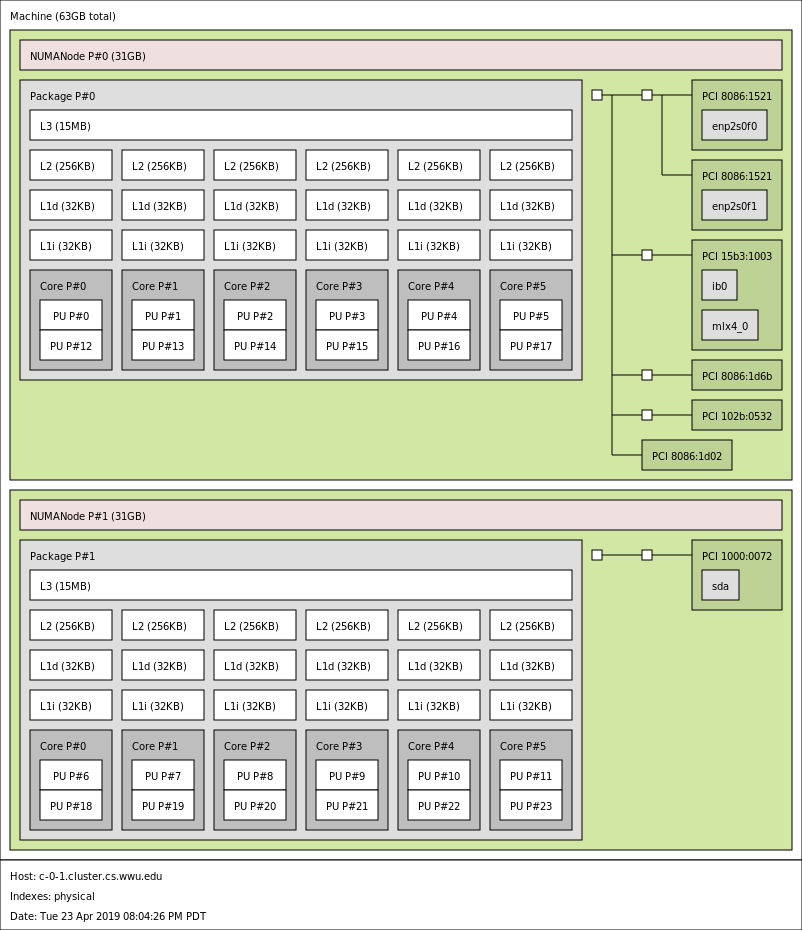
\includegraphics[width=\textwidth]{cluster}
\end{figure}


\twocolumn
\section {Thread Affinity}

\paragraph {The first program which was ran was designed to spawn 12 threads (one thread per core), and for each thread,
perform groups of computations, sequentially, on unique partitions of large amounts of data. The source code used follows.}

\subsection{Results}

\paragraph{The thread affinity program was ran 5 times consecutively.
  Each benchmark was recorded in seconds, and an average, minimum,
  and maximum amount were taken for each of them. }

\paragraph{We used the 4 standard execution profiles provided by OpenMP. Out of all of them,
  the profile which favored spreading threads throughout the cores (yet with the capability to still be spread to multiple sockets)
  performed the best.}

\begin{itemize}
  \item Average time: 0.012390 seconds
  \item Min time: 0.01235 seconds
  \item Max time: 0.012454 seconds    
\end{itemize}

\subsection{Conclusion}

\paragraph{It seems logical that the cores spread execution profile would run the fastest: we're using only one thread per core, and despite the NUMA architecture playing a pivotal role in memory access latency, the L1 caches themselves are also per-core, so any reaches out to main memory are few and far between. Furthermore, the way stride of the data for each thread is mapped reduces the need for out of socket memory reads/writes. Of course, it's worth while to consider factors such as how the NUMA architecture searches other out of socket L3 caches if the data it's searching for hasn't been found in its own L3 cache.}

\section{Matrix Multiply}

\subsection{Thread Variance}

\paragraph{The relevant code we were using for this section of the assignment is as follows.}

\paragraph{The speedup for the parallel version of the matrix gradually made its way to about 4x as the thread size increased; there are moments where a difference in the amount of threads used doesn't provide much of an increase in speedup, as is illustrated in the graph when the test is ran using between 8 and 10 threads. Apart from that, though, the speedup is fairly significant. The speedup was calculated by simply dividing the time of the serial version of the multiply against the time of the parallel version of the multiply.
Initially, attempts were made to parallelize the outer most loop as opposed to the innermost loop. The end result was along the lines of 30 seconds, irrespective of the amount of threads used.}

\begin{figure}[h]
\caption{speedup as the amount of threads are increased for each run}
\centering
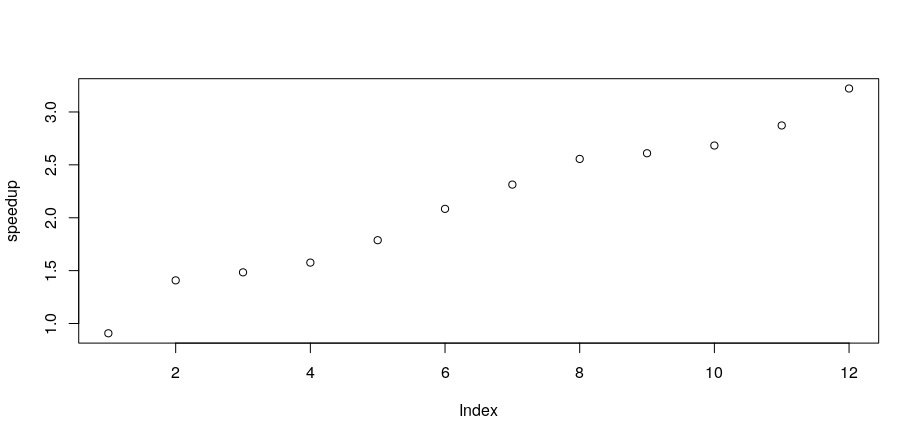
\includegraphics[width=50mm,scale=0.5]{matrix_mul_speedup}
\end{figure}

\subsection{Chunk and Schedule Policy variance}

\begin{lstlisting}[language=Python]
[
  (9.326500,6.050310),  # STATIC-10
  (9.221319,6.205454),  # STATIC-100
  (9.214018,6.008883),  # STATIC-1000
  (9.228346,5.947109),  # DYNAMIC-10
  (9.191903,6.159095),  # DYNAMIC-100
  (9.221951,6.116993),  # DYNAMIC-1000
]
\end{lstlisting}

\paragraph{The first entry in each tuple shown above is the time for the serial execution. The second is of course the time for the parallel application.
Interestingly enough, the best performance appears to be had from using the dynamic parallellization with a low chunk count. Speculatively, this would make sense considering that a single cache line can hold about 16 integers; assigning chunk sizes of 10 for the innermost loop allows for a flexible distribution of elements for each row. In general, we're more likely to have better latency and less cache conflicts, since loading and unloading cache lines will happen once for the execution of each thread (it's going to happen multiple times for sizes of the thousands or hundreds).}

\end{document}
